% Provenance (never printed): see sources/outline_sources.md (Year 1: rigid plates on a
% sphere, Euler poles and angular velocities; relative velocities; triple junctions;
% finite rotations; the magnetic-anomaly timescale; satellite geodesy). Curves and maps
% from figdata/bachelor-1/euler_velocities.py, south_atlantic_fit.py and gpts_stripes.py;
% exercise and problem values in the Book 3 scratch calculator calc/ch12.py.
\chapter{गोले पर प्लेट गतिकी}\label{ch:b1:plate-kinematics}

दो उपग्रह-स्थिति स्टेशन एक चौथाई सदी से अधिक समय से हर दिन अपनी स्थिति दर्ज कर रहे हैं: एक रेक्याविक में, पश्चिमी आइसलैंड में, दूसरा स्टैवेंगर के निकट, नॉर्वे के पश्चिमी तट पर। उनके बीच की सीधी रेखा, \qty{1546}{km} लंबी, हर वर्ष \qty{17.5}{mm} बढ़ती है, लगभग दो सेंटीमीटर। ज़मीन पर कुछ भी यह नहीं दिखाता, फिर भी दोनों स्टेशनों के बीच उत्तरी अटलांटिक का तल लाखों वर्षों से वही चौड़ाई दर्ज करता है: मध्य-अटलांटिक कटक पर निकला लावा ठंडा होते समय पृथ्वी के चुंबकीय क्षेत्र की दिशा ले लेता था, और क्षेत्र कई बार उलट चुका है, इसलिए महासागर-तल अपनी वृद्धि का एक धारीदार अभिलेख रखता है। यह अध्याय विद्यालय वर्षों की प्लेटों को गोले पर कठोर टोपियों में बदलता है, घूर्णनों की ज्यामिति से उनकी गतियों का वर्णन करता है, और दिखाता है कि भूवैज्ञानिक अभिलेख और उपग्रह एक ही गतियाँ कैसे मापते हैं।
% ledger: ngl:reyk, ngl:stas (chord lengthening computed in calc/ch12.py)

\begin{recall}
गोले पर एक \omterm{def:b1:spherical-astronomy:spherical-triangle}{महावृत्त} वह छेद है जो केंद्र से होकर गुज़रते एक तल से बनता है, एक लघुवृत्त कोई अन्य तल से; कोज्या-नियम दो बिंदुओं के बीच की कोणीय दूरी उनके अक्षांशों और देशांतरों से देता है, और एक दिशा का दिगंश उत्तर से पूर्व की ओर गिना जाता है (\cref{ch:b1:spherical-astronomy})। एक स्थिर अक्ष पर घूमते दृढ़ पिंड का एक कोणीय वेग होता है (भौतिकी)। \omterm{def:b1:layered-earth:lithosphere}{स्थलमंडल} ऐसी प्लेटों में टूटा है जो एक-दूसरे के सापेक्ष कुछ सेंटीमीटर प्रति वर्ष चलती हैं, और महासागर-तल पर चुंबकीय धारियाँ हैं जो पृथ्वी के चुंबकीय क्षेत्र के उलटावों का अभिलेख हैं (पुस्तक 2, कक्षा 11)।
\end{recall}

\section{गोले पर दृढ़ प्लेटें}

यूरेशियन प्लेट अटलांटिक के मध्य से पूर्वी साइबेरिया तक फैली है। उसकी गति एक वेग से वर्णित नहीं हो सकती, जैसे कार की गति हो सकती है; उसे एक घूर्णन से वर्णित करना होगा।

\begin{definition}[दृढ़ प्लेट]\label{def:b1:plate-kinematics:rigid-plate}
एक \emph{दृढ़ प्लेट}\index{दृढ़ प्लेट} \omterm{def:b1:layered-earth:lithosphere}{स्थलमंडल} का एक क्षेत्र है जिसका भीतरी भाग मापने योग्य रूप से विकृत नहीं होता: उसके किन्हीं दो बिंदुओं के बीच की दूरी स्थिर रहती है। दो प्लेटों की सापेक्ष गति उनकी साझा सीमा पर उठाई जाती है, दोषों, भूकंपों और ज्वालामुखियों के एक संकरे क्षेत्र में।
\end{definition}

कोई प्लेट पूर्णतः दृढ़ नहीं है: सीमाएँ दसियों से सैकड़ों किलोमीटर चौड़े क्षेत्र हैं, और भीतरी भाग धीरे विकृत होते हैं। परिकल्पना यह है कि ये विचलन सापेक्ष गतियों के सामने छोटे हैं; इस अध्याय के हर परिणाम की संगति से इसकी जाँच होती है।

गोले की सतह पर एक \omterm{def:b1:plate-kinematics:rigid-plate}{दृढ़ प्लेट} बिना किन्हीं दो बिंदुओं के बीच दूरी बदले चलती है, और पृथ्वी का केंद्र नहीं चलता। ऐसी गति एक $3\times3$ आव्यूह $R$ से वर्णित होती है जो लंबाइयाँ बनाए रखता है, एक \emph{लंबकोणीय} आव्यूह ($R^{\mathsf T}R = I$), और जो अंतरिक्ष का अभिविन्यास बनाए रखता है, ताकि $\det R = 1$ हो: स्थिति-सदिश $\vec r$ वाला एक बिंदु $R\vec r$ पर जाता है।

\begin{theorem}[यूलर का घूर्णन प्रमेय]\label{thm:b1:plate-kinematics:euler}
गोले पर दृढ़ प्लेट का हर विस्थापन पृथ्वी के केंद्र से होकर जाने वाले एक अक्ष के परितः घूर्णन है: एक इकाई सदिश $\vec n$ है जिसके लिए $R\vec n = \vec n$ है, और प्लेट $\vec n$ के परितः किसी कोण से घूमती है।
\end{theorem}

\begin{proof}
हम दिखाते हैं कि $1$, $R$ का एक आइगेनमान है, अर्थात् $\det(R - I) = 0$। चूँकि
$R R^{\mathsf T} = I$ है, हमारे पास $R - I = R(I - R^{\mathsf T})$ है, अतः
\[
  \det(R - I) = \det R\,\det\bigl((I - R)^{\mathsf T}\bigr) = \det(I - R),
\]
$\det R = 1$ का उपयोग करके, और इस तथ्य से कि एक आव्यूह और उसके परिवर्त का सारणिक एक ही है। $3\times3$ आव्यूह के लिए,
$\det(I - R) = (-1)^3\det(R - I) = -\det(R - I)$। अतः $\det(R - I) =
-\det(R - I)$ है, जो शून्य है। एक इकाई सदिश $\vec n$, जिसके लिए $R\vec n = \vec n$ है, इसलिए विद्यमान है: केंद्र से होकर $\vec n$ की दिशा में जाने वाली रेखा जहाँ सतह को काटती है वे दो बिंदु नहीं चलते। $\vec n$ के लंबवत तल में $R$ लंबाइयाँ और अभिविन्यास बनाए रखता है: वह उस तल को किसी कोण से घुमाता है, और इस तरह पूरे गोले को $\vec n$ के परितः।
\end{proof}

अंतराल पर जो गति बदले बिना पर्याप्त छोटा है, घूर्णन एक स्थिर दर से आगे बढ़ता है, और एक प्लेट की दूसरी के सापेक्ष गति एक स्थिर अक्ष के परितः एक कोणीय वेग है।

\begin{definition}[यूलर ध्रुव; यूलर सदिश]\label{def:b1:plate-kinematics:euler-pole}
प्लेट B की प्लेट A के सापेक्ष गति पृथ्वी के केंद्र से होकर जाने वाले एक अक्ष के परितः घूर्णन है। युग्म का \emph{यूलर ध्रुव}\index{यूलर ध्रुव} वह बिंदु है जहाँ यह अक्ष सतह को काटता है, इस प्रकार चुना गया कि घूर्णन उसके ऊपर से देखने पर वामावर्त हो; प्रतिध्रुवीय बिंदु विपरीत ध्रुव है। \emph{यूलर सदिश}\index{यूलर सदिश} $\vec\omega_{BA}$ B का A के सापेक्ष कोणीय वेग है: वह पृथ्वी के केंद्र से यूलर ध्रुव की ओर इंगित करता है, और उसकी लंबाई $\omega$ घूर्णन की दर है।
\end{definition}

एक \omterm{def:b1:plate-kinematics:euler-pole}{यूलर सदिश} उसके ध्रुव के \omterm{def:b1:spherical-astronomy:geographic}{अक्षांश} और \omterm{def:b1:spherical-astronomy:geographic}{देशांतर} और उसकी दर से दिया जाता है, आम तौर पर प्रति दस लाख वर्ष डिग्री में। यूरेशियन प्लेट की उत्तर अमेरिकी प्लेट के सापेक्ष गति, अंतिम \qty{3.16}{Myr} पर उनके बीच के कटकों पर मापी गई 453 प्रसार-दरों से औसत निकाली गई, का ध्रुव \ang{61.8}\,N, \ang{139.6}\,E पर है, पूर्वी साइबेरिया में, और दर \qty{0.210}{\degree\per\Myr} है। रेडियन प्रति वर्ष में,
\[
  \omega = \frac{0.210\times\pi/180}{\num{e6}} = \qty{3.665e-9}{rad.yr^{-1}},
\]
एक पूरा चक्कर \qty{1714}{\Myr} में।
% ledger: morvel:eu-na, morvel:summary

\section{सापेक्ष वेग}

\begin{theorem}[घूमती प्लेट पर वेग]\label{thm:b1:plate-kinematics:velocity}
यदि प्लेट B \omterm{def:b1:plate-kinematics:euler-pole}{यूलर सदिश} $\vec\omega$ के साथ प्लेट A के सापेक्ष घूमती है, तो B के स्थिति-सदिश $\vec r$ (पृथ्वी के केंद्र से) वाला एक बिंदु A के सापेक्ष निम्न वेग से गति करता है:
\[
  \vec v = \vec\omega\times\vec r .
\]
\end{theorem}

\begin{proof}
माना $\Delta$, $\vec\omega$ और $\vec r$ के बीच का कोण है। B के घूमने पर बिंदु अक्ष के परितः त्रिज्या $R\sin\Delta$ का एक वृत्त वर्णित करता है, जहाँ $R$ पृथ्वी की त्रिज्या है; कोणीय दर $\omega$ पर उसकी चाल $\omega R\sin\Delta$ है। उसका वेग उस वृत्त की स्पर्श-रेखा पर है, अतः अक्ष और त्रिज्या $\vec r$ दोनों के लंबवत, और घूर्णन $\vec\omega$ के परितः वामावर्त होने से उसकी दिशा $\vec\omega\times\vec r$ की है। सदिश $\vec\omega\times\vec r$ की ठीक यही दिशा और अभिविन्यास है, और लंबाई $\omega R\sin\Delta$ है।
\end{proof}

कोण $\Delta$ ध्रुव और बिंदु के बीच की कोणीय दूरी है, जिसे कोज्या-नियम अक्षांशों और देशांतरों से देता है।

\begin{proposition}[सापेक्ष गति की चाल और दिशा]\label{prop:b1:plate-kinematics:speed}
माना \omterm{def:b1:plate-kinematics:euler-pole}{यूलर ध्रुव} \omterm{def:b1:spherical-astronomy:geographic}{अक्षांश} $\varphi_p$ और \omterm{def:b1:spherical-astronomy:geographic}{देशांतर} $\lambda_p$ पर है, और बिंदु $\varphi$ और $\lambda$ पर। तब
\begin{enumerate}
  \item ध्रुव से बिंदु तक की कोणीय दूरी $\Delta$ संतुष्ट करती है
        $\cos\Delta = \sin\varphi_p\sin\varphi + \cos\varphi_p\cos\varphi
        \cos(\lambda - \lambda_p)$;
  \item सापेक्ष चाल $v = \omega R\sin\Delta$ है: ध्रुव पर शून्य, और सबसे बड़ी, $\omega R$, उससे \ang{90} दूर के \omterm{def:b1:spherical-astronomy:spherical-triangle}{महावृत्त} पर।
  \item गति की दिशा उस \omterm{def:b1:spherical-astronomy:spherical-triangle}{महावृत्त} के लंबवत है जो बिंदु को ध्रुव से जोड़ता है: उसका दिगंश, बिंदु से देखे गए ध्रुव के दिगंश के, प्लस \ang{90}, के बराबर है।
\end{enumerate}
\end{proposition}

\begin{proof}
(1) यह भौगोलिक उत्तरी ध्रुव, \omterm{def:b1:plate-kinematics:euler-pole}{यूलर ध्रुव} और बिंदु से बने \omterm{def:b1:spherical-astronomy:spherical-triangle}{गोलीय त्रिभुज} पर कोज्या-नियम है, जिसकी उत्तरी ध्रुव से भुजाएँ $\ang{90} - \varphi_p$ और $\ang{90} - \varphi$ हैं, उनके बीच कोण $\lambda - \lambda_p$ के साथ। (2) प्रमेय से आता है। (3) वेग $\vec\omega$ और $\vec r$ के लंबवत है, अतः उस तल के लंबवत जिसमें वे हैं, यानी बिंदु और ध्रुव से होकर जाने वाले \omterm{def:b1:spherical-astronomy:spherical-triangle}{महावृत्त} का तल। बिंदु पर क्षैतिज तल में वह इसलिए ध्रुव की दिशा के लंबवत है; ध्रुव के ऊपर से देखने पर घूर्णन वामावर्त होने से, बिंदु उस दिशा के दाहिनी ओर चलता है जिसमें वह ध्रुव को देखता है, जो दिगंश में \ang{90} जोड़ता है।
\end{proof}

\begin{omfigure}
\begin{tikzpicture}[x=2.5cm, y=2.5cm, font=\scriptsize, >=Stealth]
% orthographic view from 20 deg above the "Euler equator": a point at polar angle D,
% longitude p about the pole projects to X = sin D sin p, Y = cos D cos 20 - sin D cos p sin 20;
% it is visible when cos p >= -cot D tan 20 (limits computed by hand: 129.08, 102.13, 90, 77.87)
\fill[omSea!12] (0,0) circle (1);
\draw[thick] (0,0) circle (1);
\foreach \D/\m in {30/129.08, 60/102.13, 90/90, 120/77.87} {
  \draw[blue!45!black, domain=-\m:\m, samples=60, variable=\p]
    plot ({sin(\D)*sin(\p)}, {cos(\D)*cos(20) - sin(\D)*cos(\p)*sin(20)});
  \draw[blue!45!black, densely dashed, domain=\m:360-\m, samples=60, variable=\p]
    plot ({sin(\D)*sin(\p)}, {cos(\D)*cos(20) - sin(\D)*cos(\p)*sin(20)});
}
\draw[densely dashed] (0,0) -- (0,0.9397);
\draw[->, very thick] (0,0.9397) -- (0,1.38) node[above] {$\vec\omega$};
\fill (0,0.9397) circle (0.9pt) node[anchor=south west] {यूलर ध्रुव};
\fill (0,0) circle (0.7pt);
% velocity arrows at longitude -35 deg about the pole, length 0.5 sin D
\draw[->, very thick, red!75!black] (-0.287,0.6737) -- ++(0.243,-0.058);
\draw[->, very thick, red!75!black] (-0.497,0.2272) -- ++(0.421,-0.101);
\draw[->, very thick, red!75!black] (-0.574,-0.2802) -- ++(0.487,-0.117);
\draw[->, very thick, red!75!black] (-0.497,-0.7124) -- ++(0.421,-0.101);
\draw[->] (0,0) -- (-0.497,0.2272) node[pos=0.55, below] {$\vec r$};
\draw (0,0.22) arc[start angle=90, end angle=155.4, radius=0.22];
\node at (-0.11,0.33) {$\Delta$};
\node[anchor=west] at (0.62,0.81) {$\Delta = \ang{30}$};
\node[anchor=west] at (0.88,0.47) {$\Delta = \ang{60}$};
\node[anchor=west] at (1.02,0.0) {$\Delta = \ang{90}$};
\node[anchor=west] at (0.88,-0.47) {$\Delta = \ang{120}$};
\end{tikzpicture}

\par\smallskip{\small एक प्लेट अपने \omterm{def:b1:plate-kinematics:euler-pole}{यूलर ध्रुव} के परितः घूमती हुई, ध्रुव से \ang{90} दूर वृत्त के थोड़े ऊपर से देखी गई। हर बिंदु ध्रुव के परितः एक लघुवृत्त पर चलता है (छिपे भाग बिंदुकित); उसकी चाल, लाल तीरों से दिखाई गई, $\omega R\sin\Delta$ है, जहाँ $\Delta$ ध्रुव से उसकी कोणीय दूरी है: ध्रुव पर शून्य, \ang{90} दूर सबसे अधिक।}
\label{fig:b1:plate-kinematics:euler-pole}
\end{omfigure}

प्लेट सीमा के साथ सापेक्ष चाल इसलिए बदलती है, भले ही दोनों प्लेटें पूर्णतः दृढ़ हों, और गति की दिशा उसके साथ घूमती है। दो परिणाम हर प्लेट-सीमा के मानचित्र को आकार देते हैं।

\begin{proposition}[रूपांतर भ्रंश लघुवृत्तों पर चलते हैं]\label{prop:b1:plate-kinematics:transforms}
एक रूपांतर भ्रंश, जिसके साथ दो प्लेटें बिना खुले या बंद हुए एक-दूसरे को सरकती हैं, दोनों प्लेटों के \omterm{def:b1:plate-kinematics:euler-pole}{यूलर ध्रुव} के परितः एक लघुवृत्त पर स्थित है। कटक पर प्रसार की, और एक निमज्जन-क्षेत्र पर अभिसरण की दिशा भी लघुवृत्तों के अनुदिश है।
\end{proposition}

\begin{proof}
रूपांतर भ्रंश पर सापेक्ष वेग हर बिंदु पर भ्रंश के समांतर है। सापेक्ष वेग हर जगह ध्रुव के परितः लघुवृत्तों पर स्पर्श-रेखीय है (\cref{thm:b1:plate-kinematics:velocity}); उसके हर बिंदु पर उस बिंदु से होकर जाने वाले लघुवृत्त की स्पर्श-रेखा वाला वक्र इन्हीं वृत्तों में से एक है। दूसरा कथन \cref{prop:b1:plate-kinematics:speed} का तीसरा भाग है।
\end{proof}

यूरेशिया और उत्तरी अमेरिका के बीच मध्य-अटलांटिक कटक रूपांतर भ्रंशों से विस्थापित कटक-खंडों की एक सीढ़ी है; रूपांतर लगभग उन दिगंशों के निकट चलते हैं जिनकी \omterm{def:b1:plate-kinematics:euler-pole}{यूलर सदिश} भविष्यवाणी करता है, और उनकी प्रवृत्ति उन आँकड़ों में से एक है जिनसे ध्रुव खोजा गया। उसी सीमा के साथ प्रसार-दर ध्रुव से कोणीय दूरी के साथ बढ़ती है: आर्कटिक महासागर में गाक्कल कटक पर, ध्रुव के निकट, \qtyrange{11}{12}{mm.yr^{-1}}, और अज़ोरेस के ठीक उत्तर में, उससे \ang{78} दूर, \qty{23}{mm.yr^{-1}}। नीचे का चित्र सीमा के हर भाग पर \omterm{def:b1:plate-kinematics:euler-pole}{यूलर सदिश} की भविष्यवाणी की गई दरों की एक स्वतंत्र प्लेट-प्रतिरूप की दरों से तुलना करता है।
% ledger: morvel:eu-na

\begin{method}[किसी बिंदु पर वेग]\label{met:b1:plate-kinematics:velocity}
\begin{enumerate}
  \item \omterm{def:b1:plate-kinematics:euler-pole}{यूलर सदिश} की दर को रेडियन प्रति वर्ष में बदलिए, और $\omega R$ परिकलित कीजिए, \unit{mm.yr^{-1}} में $R = \qty{6371}{km}$ के साथ।
  \item कोसाइन-नियम से ध्रुव से बिंदु तक की कोणीय दूरी $\Delta$ परिकलित कीजिए; चाल $\omega R\sin\Delta$ है।
  \item बिंदु से देखे गए ध्रुव का दिगंश $\beta$ परिकलित कीजिए, $\tan\beta = \sin(\lambda_p - \lambda)\cos\varphi_p /
        \bigl(\cos\varphi\sin\varphi_p - \sin\varphi\cos\varphi_p
        \cos(\lambda_p - \lambda)\bigr)$ के साथ, और अंश और हर के चतुर्थांश के साथ; गति $\beta + \ang{90}$ की ओर है।
  \item दिशा जाँचिए: गति दूसरी प्लेट की पहली के सापेक्ष है। प्लेटों का आदान-प्रदान उसे उलट देता है।
\end{enumerate}
\end{method}

\begin{example}[आइसलैंड में यूरेशिया उत्तरी अमेरिका से दूर जाता है]\label{ex:b1:plate-kinematics:iceland}
मध्य आइसलैंड को \ang{64.5}\,N, \ang{18}\,W पर लीजिए, और ऊपर दिए यूरेशिया के उत्तरी अमेरिका के सापेक्ष \omterm{def:b1:plate-kinematics:euler-pole}{यूलर सदिश} को। तब $\omega R =
\num{3.665e-9}\times\qty{6.371e9}{mm} = \qty{23.35}{mm.yr^{-1}}$, और
\[
  \cos\Delta = \sin\ang{61.8}\sin\ang{64.5}
  + \cos\ang{61.8}\cos\ang{64.5}\cos(\ang{-18} - \ang{139.6}) = 0.60736,
\]
अतः $\Delta = \ang{52.60}$ और $v = 23.35\sin\ang{52.60} = \qty{18.55}{mm.yr^{-1}}$।
बिंदु से देखा गया ध्रुव दिगंश $\beta = \ang{13.1}$ पर है, उत्तर से थोड़ा पूर्व की ओर, आर्कटिक के ऊपर; यूरेशिया $\ang{103.1}$ की ओर चलता है, पूर्व-दक्षिण-पूर्व, अर्थात् पूर्व में \qty{18.07}{mm.yr^{-1}} और दक्षिण में \qty{4.20}{mm.yr^{-1}}।
% computed in calc/ch12.py and figdata/bachelor-1/euler_velocities.py
\end{example}

\begin{omfigure}
\begin{tikzpicture}
\begin{axis}[omrecord, width=0.84\linewidth, height=6.4cm, xmin=0, xmax=90, ymin=0, ymax=26,
  xtick={0,15,...,90}, xlabel={यूलर ध्रुव से कोणीय दूरी, $\Delta$ (डिग्री)},
  ylabel={प्रसार-दर (\unit{mm.yr^{-1}})},
  legend style={font=\scriptsize, at={(0.99,0.03)}, anchor=south east, draw=none, fill=white, fill opacity=0.85, text opacity=1},
  legend cell align=left]
% computed in figdata/bachelor-1/euler_velocities.py
\addplot[only marks, mark=*, mark size=0.9pt, black!55] table[x=delta, y=pb2002] {figdata/out/bachelor-1-euler_velocities-mar.dat};
\addlegendentry{प्लेट-सीमा प्रतिरूप PB2002, हर सीमा-चरण}
\addplot[only marks, mark=x, mark size=1.1pt, blue!60!black] table[x=delta, y=gps] {figdata/out/bachelor-1-euler_velocities-mar.dat};
\addlegendentry{उपग्रह स्थिति-निर्धारण से यूलर सदिश}
\addplot[very thick, red!75!black] table[x=delta, y=v] {figdata/out/bachelor-1-euler_velocities-curve.dat};
\addlegendentry{$\omega R\sin\Delta$, भूवैज्ञानिक यूलर सदिश}
\node[font=\scriptsize, anchor=south east] at (axis cs:52.6,19.6) {आइसलैंड};
\draw[black!70] (axis cs:52.6,18.55) circle (2.5pt);
\node[font=\scriptsize, anchor=south] at (axis cs:78.4,23.6) {अज़ोरेस};
\draw[black!70] (axis cs:78.4,22.87) circle (2.5pt);
\node[font=\scriptsize, anchor=south] (gk) at (axis cs:9,12) {गाक्कल कटक};
\draw[black!70, -{Stealth[length=3pt]}] (gk.south) -- (axis cs:16.5,7.2);
\end{axis}
\end{tikzpicture}

\par\smallskip{\small यूरेशिया और उत्तरी अमेरिका के बीच प्रसार-दरें, आर्कटिक महासागर से अज़ोरेस तक, \omterm{def:b1:plate-kinematics:euler-pole}{यूलर ध्रुव} से कोणीय दूरी के विरुद्ध। लाल: भूवैज्ञानिक \omterm{def:b1:plate-kinematics:euler-pole}{यूलर सदिश} (ध्रुव \ang{61.8}\,N, \ang{139.6}\,E, \qty{0.210}{\degree\per\Myr}), जो सारी दरों को एक ही ज्या-वक्र पर रखता है। धूसर: एक स्वतंत्र प्लेट-सीमा प्रतिरूप की दरें उसके हर सीमा-चरण पर; वे वक्र से औसतन \qty{1}{\percent} भिन्न हैं। नीला: उन्हीं चरणों पर उपग्रह स्थिति-निर्धारण से दोनों प्लेट-आंतरिक भागों में परिकलित \omterm{def:b1:plate-kinematics:euler-pole}{यूलर सदिश} से भविष्यवाणी की गई दरें (ध्रुव \ang{74.2}\,N, \ang{134.1}\,E, \qty{0.237}{\degree\per\Myr}): उसका ध्रुव अन्यत्र होने से, उसकी दरें लाल वक्र पर नहीं पड़तीं। वे अज़ोरेस से आइसलैंड तक भूवैज्ञानिक दरों के एक दसवें के भीतर हैं, और आर्कटिक में बहुत कम, जहाँ दरें छोटी हैं और ध्रुव की सटीक स्थिति पर प्रबल रूप से निर्भर।}
\label{fig:b1:plate-kinematics:mar-rates}
\end{omfigure}
% ledger: morvel:eu-na, morvel:gps-eu-na, data:pb2002 (mean difference 0.96 per cent, euler_velocities.py)

\section{गतियों का संयोजन; त्रि-संधियाँ}

सापेक्ष वेग यांत्रिकी के वेगों की तरह जुड़ते हैं: यदि B, A के सापेक्ष चलता है और C, B के सापेक्ष, तो C, A के सापेक्ष दोनों वेगों के योग से चलता है।

\begin{proposition}[यूलर सदिश जुड़ते हैं]\label{prop:b1:plate-kinematics:addition}
तीन प्लेटों A, B, C के लिए,
\[
  \vec\omega_{CA} = \vec\omega_{CB} + \vec\omega_{BA}, \qquad
  \vec\omega_{AB} = -\vec\omega_{BA}.
\]
\end{proposition}

\begin{proof}
हर बिंदु $\vec r$ पर, $\vec v_{CA} = \vec v_{CB} + \vec v_{BA}$, अर्थात्
$\vec\omega_{CA}\times\vec r = \vec\omega_{CB}\times\vec r +
\vec\omega_{BA}\times\vec r = (\vec\omega_{CB} + \vec\omega_{BA})\times\vec r$
सदिश गुणनफल की रैखिकता से। एक सदिश $\vec u$ जिसके लिए $\vec u\times\vec r = \vec 0$ हर $\vec r$ के लिए है, शून्य है, अतः दोनों \omterm{def:b1:plate-kinematics:euler-pole}{यूलर सदिश} बराबर हैं। A और B का आदान-प्रदान हर वेग को उलट देता है।
\end{proof}

यूलर सदिशों को जोड़ने के लिए हर एक को कार्तीय घटकों में लिखिए, $\omega(\cos\varphi_p
\cos\lambda_p, \cos\varphi_p\sin\lambda_p, \sin\varphi_p)$, घटक जोड़िए, और एक ध्रुव और एक दर में वापस बदलिए। ध्रुव जोड़े नहीं जा सकते; \omterm{def:b1:plate-kinematics:euler-pole}{यूलर सदिश} जोड़े जा सकते हैं। यह संबंध एक शक्तिशाली बाधा है। नूबियन प्लेट (अफ्रीका) की यूरेशिया के सापेक्ष गति धीमी है, और भूवैज्ञानिक अभिलेख उसके कुछ सीधे माप देता है: अज़ोरेस और जिब्राल्टर के बीच, एकमात्र माप एक ही रूपांतर, ग्लोरिया भ्रंश, के दिगंश हैं। वह इसके बजाय अटलांटिक के आर-पार दो अच्छी तरह मापी गई प्रसार-गतियों से आती है: $\vec\omega_{\mathrm{NB\,NA}}$ (ध्रुव \ang{79.2}\,N, \ang{40.2}\,E, \qty{0.233}{\degree\per\Myr}) के साथ और ऊपर की $\vec\omega_{\mathrm{EU\,NA}}$ के साथ, $\vec\omega_{\mathrm{NB\,EU}} =
\vec\omega_{\mathrm{NB\,NA}} - \vec\omega_{\mathrm{EU\,NA}}$ का ध्रुव \ang{20.9}\,N, \ang{18.3}\,W पर है, पश्चिम अफ्रीका के तट से दूर, और दर \qty{0.123}{\degree\per\Myr} (\cref{exo:b1:plate-kinematics:7})।
% ledger: morvel:nb-na, morvel:eu-na, morvel:nb-eu

\begin{definition}[त्रि-संधि; स्थायी त्रि-संधि]\label{def:b1:plate-kinematics:triple-junction}
एक \emph{त्रि-संधि}\index{त्रि-संधि} वह बिंदु है जहाँ तीन प्लेटें मिलती हैं, और उनके साथ तीन प्लेट-सीमाएँ, प्रत्येक एक कटक (R), एक खाई (T) या एक रूपांतर भ्रंश (F)। एक त्रि-संधि \emph{स्थायी}\index{स्थायी त्रि-संधि} है यदि, प्लेटों के चलने पर, वह अपनी ज्यामिति बनाए रखती है: उन्हीं तीन प्रकार की सीमाएँ उन्हीं कोणों पर मिलती हुईं।
\end{definition}

हर सीमा संधि को उसकी ज्यामिति बदले बिना केवल कुछ तरीकों से चलने देती है। एक सममित कटक अपनी दो प्लेटों के बीच मध्य में रहता है; एक रूपांतर अपनी दिशा बनाए रखता है, चाहे संधि उसके अनुदिश कुछ भी करे; एक खाई अपनी ऊपरी प्लेट से जुड़ी रहती है। प्रश्न यह है कि क्या संधि की एक गति तीनों सीमाओं को एक साथ संतुष्ट करती है। इसका उत्तर \emph{वेग-अंतरिक्ष} में दिया जाता है: एक आरेख जिसमें हर प्लेट एक बिंदु है जिसका स्थिति-सदिश संधि पर प्लेट का वेग है, किसी एक प्लेट के सापेक्ष, ताकि दो बिंदुओं को जोड़ने वाली भुजा दो प्लेटों की सापेक्ष गति हो।

\begin{proposition}[कटक–कटक–कटक संधियाँ स्थायी हैं]\label{prop:b1:plate-kinematics:rrr}
तीन कटकों की एक संधि, जिनमें से हर एक अपनी धुरी के सममित और लंबवत प्रसार करता है, तीनों प्लेटों के सापेक्ष वेग चाहे जो हों, \omterm{def:b1:plate-kinematics:triple-junction}{स्थायी} है।
\end{proposition}

\begin{proof}
माना $a$, $b$, $c$ वेग-अंतरिक्ष में तीन प्लेटों के बिंदु हैं। A और B के बीच एक कटक जो सममित रूप से प्रसार करता है, अपनी दो प्लेटों के माध्य वेग, $(a + b)/2$, पर चलता है, प्लस अपनी धुरी के अनुदिश कोई भी वेग, जो $ab$ के लंबवत है: संधि के वे वेग जो कटक को अपरिवर्तित छोड़ते हैं, भुजा $ab$ का लंबद्विभाजक बनाते हैं। संधि अपनी ज्यामिति बनाए रखती है यदि उसका वेग एक साथ तीनों लंबद्विभाजकों पर हो। त्रिभुज के तीन लंबद्विभाजक सदा एक बिंदु पर मिलते हैं, उसके परिवृत्त का केंद्र। अतः संधि का एक वेग सदा विद्यमान है।
\end{proof}

मैकेंज़ी और मॉर्गन, जिन्होंने 1969 में \omterm{def:b1:plate-kinematics:triple-junction}{स्थायी} और अस्थायी संधियों के बीच भेद प्रस्तुत किया, संयोजनों का इसी तरह विश्लेषण किया। एक रूपांतर संधि को केवल अपने ही अनुदिश चलने देता है, अर्थात् उसकी दो प्लेटों के बिंदुओं से होकर जाने वाली रेखा के अनुदिश: अतः तीन रूपांतरों की एक संधि कभी \omterm{def:b1:plate-kinematics:triple-junction}{स्थायी} नहीं होती, क्योंकि त्रिभुज की भुजाओं से होकर जाने वाली तीन रेखाओं का कोई उभयनिष्ठ बिंदु नहीं होता। अन्य प्रकारों के लिए, स्थायित्व सीमाओं की दिशाओं और सापेक्ष वेगों पर शर्तें लगाता है।
% ledger: mckenzie:triple-junctions

\begin{omfigure}
\begin{tikzpicture}[font=\scriptsize, >=Stealth]
% (a) map view of an RRR junction, ridges perpendicular to the sides of the
% velocity triangle in (b): ray directions 110.6, -121.0, -10.8 degrees
\begin{scope}[x=1cm, y=1cm]
  \node[font=\small] at (0,2.25) {(क) मानचित्र};
  \fill[omSea!12] (-2.4,-2.0) rectangle (2.4,2.0);
  \draw[ridge] (0,0) -- (110.6:2.0);
  \draw[ridge] (0,0) -- (-121.0:2.1);
  \draw[ridge] (0,0) -- (-10.8:2.3);
  \fill (0,0) circle (1.5pt) node[anchor=south west] {J};
  \node[font=\normalsize] at (-1.5,0.3) {A};
  \node[font=\normalsize] at (1.4,1.1) {B};
  \node[font=\normalsize] at (0.7,-1.4) {C};
  \draw[->, thick] ($(110.6:1.3)+(20.6:0.12)$) -- ++(20.6:0.45);
  \draw[->, thick] ($(110.6:1.3)+(200.6:0.12)$) -- ++(200.6:0.45);
  \draw[->, thick] ($(-121:1.3)+(-31:0.12)$) -- ++(-31:0.45);
  \draw[->, thick] ($(-121:1.3)+(149:0.12)$) -- ++(149:0.45);
  \draw[->, thick] ($(-10.8:1.5)+(-100.8:0.12)$) -- ++(-100.8:0.45);
  \draw[->, thick] ($(-10.8:1.5)+(79.2:0.12)$) -- ++(79.2:0.45);
\end{scope}
% (b) velocity space: a(0,0), b(2.4,0.9), c(2.0,-1.2); circumcentre (1.365, 0.009)
\begin{scope}[xshift=5.6cm, yshift=-0.2cm, x=1.25cm, y=1.25cm]
  \node[font=\small] at (1.2,1.95) {(ख) वेग-अंतरिक्ष};
  \draw[thick] (0,0) -- (2.4,0.9) -- (2.0,-1.2) -- cycle;
  \fill (0,0) circle (1.5pt) node[left] {$a$};
  \fill (2.4,0.9) circle (1.5pt) node[above right] {$b$};
  \fill (2.0,-1.2) circle (1.5pt) node[below right] {$c$};
  \draw[omRidge!80!black, densely dashed] ($(1.365,0.009)+(-0.351*1.4,0.936*1.4)$) -- ($(1.365,0.009)+(0.351*0.9,-0.936*0.9)$);
  \draw[omRidge!80!black, densely dashed] ($(1.365,0.009)+(0.982*1.5,-0.187*1.5)$) -- ($(1.365,0.009)+(-0.982*0.6,0.187*0.6)$);
  \draw[omRidge!80!black, densely dashed] ($(1.365,0.009)+(-0.514*1.6,-0.857*1.6)$) -- ($(1.365,0.009)+(0.514*0.6,0.857*0.6)$);
  \fill[omRidge!80!black] (1.365,0.009) circle (1.6pt);
  \node[anchor=north, omRidge!80!black] at (1.30,-0.05) {$j$};
  \node[anchor=south east] at (1.05,0.50) {$ab$};
\end{scope}
\end{tikzpicture}

\par\smallskip{\small तीन प्लेटों A, B और C के बीच तीन कटकों की एक संधि J। (क) मानचित्र: हर कटक (दोहरी रेखा) अपनी धुरी के लंबवत प्रसार करता है (तीर)। (ख) वेग-अंतरिक्ष: हर प्लेट एक बिंदु है; भुजा $ab$, B का A के सापेक्ष वेग है, उनके बीच के कटक के लंबवत। वे संधि-वेग जो एक सममित कटक को अपरिवर्तित छोड़ते हैं, संगत भुजा का लंबद्विभाजक (बिंदुकित) बनाते हैं; तीनों लंबद्विभाजक सदा $j$ पर मिलते हैं, संधि का वेग।}
\label{fig:b1:plate-kinematics:rrr}
\end{omfigure}

अज़ोरेस \omterm{def:b1:plate-kinematics:triple-junction}{त्रि-संधि}, लगभग \ang{39.4}\,N, \ang{29.8}\,W पर, जहाँ उत्तरी अमेरिकी, यूरेशियन और नूबियन प्लेटें मिलती हैं, एक कटक–कटक–कटक संधि है: मध्य-अटलांटिक कटक उसके उत्तर और दक्षिण में चलता है, और धीमी टर्सीरा दरार उससे पूर्व-दक्षिण-पूर्व की ओर चलती है। संधि पर उत्तरी अमेरिकी युग्म के दो \omterm{def:b1:plate-kinematics:euler-pole}{यूलर सदिश} यूरेशिया को \qty{22.9}{mm.yr^{-1}} \ang{95} की ओर और नूबिया को \qty{19.2}{mm.yr^{-1}} \ang{104} की ओर देते हैं; अतः यूरेशिया नूबिया से \qty{4.9}{mm.yr^{-1}} पर \ang{59} की ओर दूर जाता है, टर्सीरा दरार के आरपार एक पूर्व-उत्तर-पूर्व–पश्चिम-दक्षिण-पश्चिम विस्तार। वास्तविक संधि एक बिंदु नहीं है: कटक के साथ प्रसार-दर \ang{40}\,N पर \qty{22.9}{mm.yr^{-1}} से घटकर \ang{38}\,N पर \qty{19.8}{mm.yr^{-1}} तक धीरे-धीरे गिरती है, तीन बड़ी प्लेटों के बीच फँसी लगभग \qty{100}{km} चौड़ी एक छोटी प्लेट, अज़ोरेस माइक्रोप्लेट, के आरपार।
% ledger: morvel:azores, data:pb2002 (junction point at 39.40 N, 29.77 W, three spreading boundaries), morvel:nb-eu, morvel:eu-na, morvel:nb-na (velocities computed in calc/ch12.py)

\section{परिमित घूर्णन}

\omterm{def:b1:plate-kinematics:euler-pole}{यूलर सदिश} अब की गति वर्णित करता है, कुछ मिलियन वर्षों पर औसत। प्लेटों को बहुत पहले जहाँ थीं वहाँ वापस रखने के लिए, उस घूर्णन की आवश्यकता है जो एक प्लेट को उसकी वर्तमान स्थिति से उसकी पिछली स्थिति तक ले जाए।

\begin{definition}[परिमित घूर्णन]\label{def:b1:plate-kinematics:finite-rotation}
एक \emph{परिमित घूर्णन}\index{परिमित घूर्णन} गोले का वह घूर्णन है, जो एक ध्रुव (\omterm{def:b1:spherical-astronomy:geographic}{अक्षांश}, \omterm{def:b1:spherical-astronomy:geographic}{देशांतर}) और एक कोण से दिया जाता है, और जो एक प्लेट, या उसके किनारे के एक भाग, को उसकी वर्तमान स्थिति से दूसरी प्लेट के सापेक्ष किसी दिए समय की उसकी स्थिति तक ले जाता है। एक धनात्मक कोण ध्रुव के ऊपर से देखने पर वामावर्त घुमाता है।
\end{definition}

\begin{proposition}[रॉड्रिग्ज़ का सूत्र]\label{prop:b1:plate-kinematics:rodrigues}
कोण $\alpha$ का घूर्णन, इकाई सदिश $\vec n$ के परितः, सदिश $\vec r$ को ले जाता है
\[
  \vec r\,' = \cos\alpha\,\vec r + (1 - \cos\alpha)(\vec n\cdot\vec r)\,\vec n
  + \sin\alpha\,\vec n\times\vec r .
\]
\end{proposition}

\begin{proof}
$\vec r$ को अक्ष के अनुदिश उसके भाग में बाँटिए, $\vec r_\parallel =
(\vec n\cdot\vec r)\vec n$, जिसे घूर्णन नहीं बदलता, और उसके लंबवत भाग, $\vec r_\perp = \vec r - \vec r_\parallel$ में। सदिश $\vec n\times\vec r = \vec n\times\vec r_\perp$ की लंबाई $\vec r_\perp$ की है, वह उसके और $\vec n$ के लंबवत है, और $\vec n$ के परितः उससे \ang{90} वामावर्त घूमा हुआ है। 
$\vec n$ के लंबवत तल में, कोण $\alpha$ का घूर्णन $\vec r_\perp$ को $\cos\alpha\,\vec r_\perp +
\sin\alpha\,\vec n\times\vec r$ तक ले जाता है। $\vec r_\parallel$ जोड़ने पर $\vec r\,' =
\vec r_\parallel + \cos\alpha(\vec r - \vec r_\parallel) + \sin\alpha\,
\vec n\times\vec r$ मिलता है, जो सूत्र है।
\end{proof}

सूत्र $\vec r$ में रैखिक है; आव्यूहों से लिखने पर, $\vec r\,' = R\vec r$ के साथ
\[
  R = \cos\alpha\,I + (1 - \cos\alpha)\,\vec n\,\vec n^{\mathsf T}
  + \sin\alpha
  \begin{pmatrix} 0 & -n_z & n_y\\ n_z & 0 & -n_x\\ -n_y & n_x & 0\end{pmatrix},
\]
एक लंबकोणीय आव्यूह, जिसका सारणिक $1$ है, जैसा यूलर का प्रमेय माँगता है। उसका ट्रेस $1 + 2\cos\alpha$ है, जो किसी भी घूर्णन आव्यूह का कोण देता है
(\cref{exo:b1:plate-kinematics:10})।

\omterm{def:b1:plate-kinematics:finite-rotation}{परिमित घूर्णन} क्रम-विनिमेय नहीं होते। \ang{0}\,N, \ang{0}\,E पर बिंदु को, $x$ अक्ष पर, उत्तरी ध्रुव के परितः \ang{90} से घुमाइए: वह \ang{0}\,N, \ang{90}\,E पर, $y$ अक्ष पर जाता है; फिर $x$ अक्ष के परितः \ang{90} से: वह उत्तरी ध्रुव पर पहुँचता है। दूसरे क्रम में, पहला घूर्णन बिंदु को वहीं छोड़ता है और दूसरा उसे \ang{0}\,N, \ang{90}\,E पर ले जाता है (\cref{exo:b1:plate-kinematics:8})। इसलिए प्लेट-गतियों के क्रम को आव्यूहों को सही क्रम में गुणा करके संयोजित करना होगा, कभी कोणों को जोड़कर नहीं; केवल कोणीय वेग, जो अनंत सूक्ष्म घूर्णनों का वर्णन करते हैं, सदिशों की तरह जुड़ते हैं।

\begin{omfigure}
\begin{tikzpicture}
\begin{axis}[axis equal image, width=0.8\linewidth, xmin=-85, xmax=55, ymin=-58, ymax=38,
  xtick={-80,-60,...,40}, ytick={-40,-20,0,20},
  xticklabel={$\pgfmathprintnumber{\tick}^\circ$}, yticklabel={$\pgfmathprintnumber{\tick}^\circ$},
  tick label style={font=\scriptsize}, axis background/.style={fill=omSea!10},
  unbounded coords=jump]
% computed in figdata/bachelor-1/south_atlantic_fit.py
\addplot[fill=omHypsLandC!60, draw=black!60, line width=0.3pt] table[x=lon, y=lat] {figdata/out/bachelor-1-south_atlantic_fit-af.dat};
\addplot[draw=black, line width=0.5pt] table[x=lon, y=lat] {figdata/out/bachelor-1-south_atlantic_fit-sa.dat};
\addplot[draw=blue!60!black, densely dashed, line width=0.6pt] table[x=lon, y=lat] {figdata/out/bachelor-1-south_atlantic_fit-sa84.dat};
\addplot[fill=red!40, fill opacity=0.55, draw=red!70!black, line width=0.5pt] table[x=lon, y=lat] {figdata/out/bachelor-1-south_atlantic_fit-sa120.dat};
\addplot[red!70!black, thick, densely dotted, -{Stealth}] table[x=lon, y=lat] {figdata/out/bachelor-1-south_atlantic_fit-track.dat};
\fill (axis cs:-34.9,-8.05) circle (1.6pt);
  \node[font=\scriptsize, anchor=south east, fill=white, fill opacity=0.8, text opacity=1, inner sep=1pt] at (axis cs:-36,-7) {रेसिफ़े};
  \node[font=\scriptsize, align=center] at (axis cs:-60,-17) {दक्षिण अमेरिका\\आज};
\node[font=\scriptsize, blue!60!black, anchor=east] at (axis cs:-31,-46) {83.5 Ma};
\node[font=\scriptsize, red!60!black, fill=white, fill opacity=0.8, text opacity=1, inner sep=1pt] at (axis cs:-8,-22) {120.6 Ma};
  \node[font=\scriptsize] at (axis cs:22,12) {अफ्रीका};
\end{axis}
\end{tikzpicture}

\par\smallskip{\small दक्षिण अटलांटिक का बंद होना। दक्षिण अमेरिका (काली रूपरेखा) अफ्रीका के सापेक्ष दो प्रकाशित परिमित घूर्णनों द्वारा पीछे ले जाई जाती है: \qty{83.5}{Ma} पर अपनी स्थिति तक (ध्रुव \ang{61.88}\,N, \ang{34.26}\,W, कोण \ang{33.51}; बिंदुकित), और \qty{120.6}{Ma} पर, जब महासागर खुलना शुरू हुआ (ध्रुव \ang{51.28}\,N, \ang{33.67}\,W, कोण \ang{52.35}; लाल)। बिंदुकित रेखा रेसिफ़े का अपने पुराने ध्रुव के परितः लघुवृत्त पर पथ है। \omterm{def:b1:spherical-astronomy:geographic}{अक्षांश} और \omterm{def:b1:spherical-astronomy:geographic}{देशांतर} एक वर्गाकार ग्रिड के रूप में खींचे गए हैं, जो भूमध्य रेखा से दूर आकारों को फैलाता है। तटरेखाएँ: Natural Earth।}
\label{fig:b1:plate-kinematics:south-atlantic}
\end{omfigure}
% ledger: heine:sam-saf, data:ne-land

दक्षिण अमेरिका और अफ्रीका के तटों का मिलान, जो मानचित्रों पर लंबे समय से देखा गया, अब एक गणना बन जाता है। \qty{120.6}{Ma} के घूर्णन के साथ, रेसिफ़े के निकट उत्तर-पूर्वी ब्राज़ील का तट (\ang{8.05}\,S, \ang{34.9}\,W) अपने लघुवृत्त पर लगभग \qty{5000}{km} की यात्रा के बाद गिनी की खाड़ी के तट पर \ang{3.4}\,N, \ang{8.3}\,E पर आता है: लगभग \qty{40}{mm.yr^{-1}} का औसत खुलाव। मिलान हर जगह सही नहीं है: महासागर खुलने से पहले लगभग चौदह मिलियन वर्षों तक दोनों महाद्वीप धीरे-धीरे अलग खिंचे जा रहे थे, और एक कसी पुनर्रचना को पहले दोनों ओर के खिंचे हुए किनारों और दरार-द्रोणियों को पुनःस्थापित करना होगा।
% ledger: heine:sam-saf, heine:fit (Recife computed in south_atlantic_fit.py and calc/ch12.py)

\begin{history}[गोले पर विवर्तनिकी]
1965 में एडवर्ड बुलार्ड और दो सहकर्मियों ने एक न्यूनतम-वर्ग कसौटी से कंप्यूटर द्वारा अटलांटिक के चारों ओर के महाद्वीपों को फ़िट किया: सर्वोत्तम मिलान महाद्वीपीय किनारे के तीखे भाग का अनुसरण करता है, 500 फ़ेदम (लगभग \qty{900}{m}) की गहराई पर, तटरेखा पर नहीं। उसी वर्ष टूज़ो विल्सन ने दोषों का एक नया वर्ग वर्णित किया, रूपांतर भ्रंश, और महाद्वीपीय विस्थापन पर उनका प्रभाव। 1967 में डैन मैकेंज़ी और रॉबर्ट पार्कर ने, उत्तरी प्रशांत को अपना उदाहरण लेकर, दिखाया कि सतह के भूकंप-रहित क्षेत्र गोले पर दृढ़ प्लेटों की तरह चलते हैं। 1968 में जेसन मॉर्गन ने सतह को कटकों, खाइयों और बड़े दोषों से घिरे भू-पर्पटी खंडों के रूप में वर्णित किया, और ज़ेवियर ली पिचोन ने समुद्र-तल प्रसार को महाद्वीपीय विस्थापन से जोड़ा। तीन वर्षों के भीतर, महाद्वीपों का विस्थापन गोले पर दृढ़ टोपियों की गतिकी बन गया।
% ledger: bullard:fit, wilson:transform, mckenzie:sphere, morgan:blocks, lepichon:spreading
\end{history}

\section{प्लेट गतियों का मापन}

\subsection*{महासागर-तल का चुंबकीय अभिलेख}

कटक पर निकला लावा ठंडा होते समय उस क्षण की पृथ्वी के क्षेत्र की दिशा में चुंबकत्व ले लेता है, और कटक से दूर जाते समय उसे बनाए रखता है। क्योंकि क्षेत्र अनियमित अंतरालों पर उलटता है, महासागर-तल कटक के समांतर पट्टियों में, बदलती दिशाओं में चुंबकित होता है।

\begin{definition}[समुद्री चुंबकीय विसंगति; ध्रुवता कालखंड; ध्रुवता समय-पैमाना]\label{def:b1:plate-kinematics:magnetic-anomaly}
एक \emph{समुद्री चुंबकीय विसंगति}\index{समुद्री चुंबकीय विसंगति} समुद्र में मापी गई चुंबकीय क्षेत्र की तीव्रता और उसी स्थान पर पृथ्वी के मुख्य क्षेत्र के एक संदर्भ प्रतिरूप की तीव्रता के बीच का अंतर है: वह वर्तमान क्षेत्र की दिशा में चुंबकित \omterm{def:b1:layered-earth:layers}{भूपर्पटी} के ऊपर धनात्मक है, और विपरीत दिशा में चुंबकित \omterm{def:b1:layered-earth:layers}{भूपर्पटी} के ऊपर ऋणात्मक। एक \emph{ध्रुवता कालखंड}\index{ध्रुवता कालखंड} समय का वह अंतराल है जिसमें क्षेत्र ने एक ध्रुवता रखी, जिसे एक संख्या और अक्षर n (सामान्य, जैसा आज) या r (उलटा) से नामित किया जाता है। \emph{भू-चुंबकीय ध्रुवता समय-पैमाना}\index{भू-चुंबकीय ध्रुवता समय-पैमाना} ध्रुवता कालखंडों का उनकी सीमाओं की आयुओं सहित क्रम है।
\end{definition}

समय-पैमाना ज़मीन पर और गहरे-समुद्री अवसाद-कोरों में उलटाव-क्रमों की तिथि निर्धारण से, और महासागर-तल की विसंगतियों के प्रतिरूप का मिलान करके बनता है, जिनकी चौड़ाइयाँ कालखंडों की सापेक्ष अवधियाँ बनाए रखती हैं। वर्तमान सामान्य कालखंड, C1n, \qty{0.781}{Ma} पर आरंभ हुआ, और क्षेत्र अनियमित अंतरालों पर उलटा है: समय-पैमाना अंतिम ग्यारह मिलियन वर्षों में पच्चीस सामान्य अंतराल गिनता है, कुछ एक मिलियन वर्ष से अधिक तक चलते हैं, दूसरे दस हज़ार वर्ष से थोड़े अधिक। नीचे का चित्र उस इतिहास को क्रॉन C5n के अंत तक दिखाता है, और उन पट्टियों को भी जो वह एक धीमे और एक तेज़ कटक के तल पर लिखता है।
% ledger: iodp:gpts2004

\begin{omfigure}
\begin{tikzpicture}
\begin{axis}[name=gpts, width=0.9\linewidth, height=2.3cm, xmin=0, xmax=11.04, ymin=0, ymax=1,
  ytick=\empty, xtick={0,1,...,11}, tick label style={font=\scriptsize}, axis on top,
  xlabel={आयु (Ma)}, label style={font=\scriptsize}, title={(क) ध्रुवता समय-पैमाना, \qtyrange{0}{11}{Ma}},
  title style={font=\small, yshift=-1.5ex}]
% computed in figdata/bachelor-1/gpts_stripes.py
\addplot[const plot, fill=black, draw=none] table[x=age, y=pol] {figdata/out/bachelor-1-gpts_stripes-gpts.dat} \closedcycle;
\node[font=\scriptsize, fill=white, inner sep=1pt] at (axis cs:0.39,0.5) {C1n};
\node[font=\scriptsize, fill=white, inner sep=1pt] at (axis cs:3.1,0.5) {C2An};
\node[font=\scriptsize, fill=white, inner sep=1pt] at (axis cs:4.75,0.5) {C3n};
\node[font=\scriptsize, fill=white, inner sep=1pt] at (axis cs:10.42,0.5) {C5n};
\end{axis}
\begin{axis}[name=slow, at={(gpts.south west)}, anchor=north west, yshift=-1.75cm, width=0.9\linewidth,
  height=2.3cm, xmin=-110.4, xmax=110.4, ymin=0, ymax=1, ytick=\empty, xtick={-100,-50,0,50,100},
  tick label style={font=\scriptsize}, axis on top, xlabel={कटक-अक्ष से दूरी (km)},
  label style={font=\scriptsize}, title={(ख) अर्ध प्रसार-दर \qty{10}{mm.yr^{-1}}},
  title style={font=\small, yshift=-1.5ex}]
\addplot[const plot, fill=black, draw=none] table[x=x, y=pol] {figdata/out/bachelor-1-gpts_stripes-stripes10.dat} \closedcycle;
\draw[red!80!black, very thick] (axis cs:0,0) -- (axis cs:0,1);
\end{axis}
\begin{axis}[at={(slow.south west)}, anchor=north west, yshift=-1.75cm, width=0.9\linewidth,
  height=2.3cm, xmin=-441.6, xmax=441.6, ymin=0, ymax=1, ytick=\empty, xtick={-400,-200,0,200,400},
  tick label style={font=\scriptsize}, axis on top, xlabel={कटक-अक्ष से दूरी (km)},
  label style={font=\scriptsize}, title={(ग) अर्ध प्रसार-दर \qty{40}{mm.yr^{-1}}},
  title style={font=\small, yshift=-1.5ex}]
\addplot[const plot, fill=black, draw=none] table[x=x, y=pol] {figdata/out/bachelor-1-gpts_stripes-stripes40.dat} \closedcycle;
\draw[red!80!black, very thick] (axis cs:0,0) -- (axis cs:0,1);
\end{axis}
\end{tikzpicture}

\par\smallskip{\small (क) पिछले \qty{11}{Myr} का \omterm{def:b1:plate-kinematics:magnetic-anomaly}{भू-चुंबकीय ध्रुवता समय-पैमाना} (काला: सामान्य ध्रुवता, जैसा आज; सफ़ेद: उलटा), 2004 समय-पैमाने की आयुओं सहित, छोटे उपकालखंडों सहित। (ख) और (ग) वह महासागर-तल जो एक कटक (लाल) उसी समय में, सममित रूप से प्रसार करते हुए बनाता है: हर ध्रुवता अंतराल दोनों पार्श्वों पर एक-एक धारी का एक युग्म बन जाता है, जिसकी चौड़ाई \omterm{def:b1:plate-kinematics:spreading-rate}{अर्ध प्रसार-दर} गुना उसकी अवधि के बराबर है। चार गुनी दर पर वही प्रतिरूप चार गुना चौड़ा है; जरामिलो (लगभग \qty{1}{Ma} के निकट) जैसी छोटी घटनाएँ धीमे कटक पर \qty{1}{km} से कम चौड़ी धारियाँ बनाती हैं।}
\label{fig:b1:plate-kinematics:stripes}
\end{omfigure}

\begin{definition}[अर्ध और पूर्ण प्रसार-दरें]\label{def:b1:plate-kinematics:spreading-rate}
कटक पर, किसी पार्श्व की \emph{अर्ध प्रसार-दर}\index{अर्ध प्रसार-दर} उस पार्श्व की \omterm{def:b1:layered-earth:layers}{भूपर्पटी} के कटक-अक्ष से दूर जाने की दर है। \emph{पूर्ण प्रसार-दर}\index{पूर्ण प्रसार-दर} वह दर है जिस पर दो प्लेटें एक-दूसरे से दूर जाती हैं, दो अर्ध दरों का योग; सममित प्रसार में यह अर्ध दर का दोगुना है।
\end{definition}

\begin{method}[चुंबकीय विसंगतियों से एक प्रसार-दर]\label{met:b1:plate-kinematics:rate}
\begin{enumerate}
  \item कटक के लंबवत एक चुंबकीय परिच्छेदिका पर, दोनों पार्श्वों पर विसंगतियों का क्रम चौड़ी और संकरी धारियों के प्रतिरूप से पहचानिए, और उसे ध्रुवता समय-पैमाने से मिलाइए।
  \item हर पार्श्व पर उसी कालखंड-सीमा तक अक्ष से दूरी मापिए, और उसकी आयु से भाग दीजिए: ये दो अर्ध प्रसार-दरें हैं, तब से औसत। पूर्ण दर उनका योग है, या दोनों सीमाओं के बीच की दूरी उसकी आयु से भाग।
  \item एक पुरानी सीमा को एक नई सीमा पर प्राथमिकता दीजिए: दूरी में एक किलोमीटर की त्रुटि सौ किलोमीटर की दूरी पर दस की दूरी की तुलना में कम भारित होती है।
  \item यदि परिच्छेदिका कटक के लंबवत नहीं है, तो दूरियों को प्रसार की दिशा पर प्रक्षेपित कीजिए।
\end{enumerate}
\end{method}

तीसरा बिंदु केवल पाठ-त्रुटि का प्रश्न नहीं है। \omterm{def:b1:layered-earth:layers}{भूपर्पटी} अपना चुंबकत्व एक ही रेखा के अनुदिश नहीं पाती: लावा सटे हुए, थोड़े पुराने \omterm{def:b1:layered-earth:layers}{भूपर्पटी} पर बहता है, डाइक उसमें घुसते हैं, और निचली \omterm{def:b1:layered-earth:layers}{भूपर्पटी} ऊपरी की तुलना में बाद में चुंबकित होती है। ये सभी प्रक्रियाएँ पट्टियों की सीमाओं को अक्ष से दूर खिसकाती हैं, ताकि एक ही आयु की दो सीमाओं के बीच की दूरी वास्तव में बनी \omterm{def:b1:layered-earth:layers}{भूपर्पटी} की चौड़ाई से अधिक हो। दोनों ओर का यह विस्थापन अधिकांश कटकों पर अधिकतम \qtyrange{1}{3}{km} है और रेक्यनीस कटक पर \qty{5.0}{km} तक पहुँचता है। सावधान संकलन इस बाहरी विस्थापन के लिए दरों को नीचे की ओर सुधारते हैं, \qtyrange{0.6}{2.6}{mm.yr^{-1}} तक, और उन्हें धीमे कटकों पर अंतिम \qty{3.16}{Myr} पर, कालखंड C2An की विसंगतियों तक, और तेज़ों पर \qty{0.78}{Myr} पर औसत करते हैं। गाक्कल कटक पर, जिसमें मैग्मा की कमी है, लघु जरामिलो उपकालखंड और कालखंड C2n की विसंगतियाँ अनुपस्थित हैं, जबकि आइसलैंड के दक्षिण के रेक्यनीस कटक पर, जो \qty{20}{mm.yr^{-1}} से कम पर प्रसार करता है पर मैग्मा की प्रचुर आपूर्ति के साथ, वे स्पष्ट पहचानी जाती हैं।
% ledger: morvel:summary, morvel:profiles, morvel:outward

\subsection*{उपग्रह भू-मिति}

1990 के दशक से \omterm{def:b1:plate-kinematics:triple-junction}{स्थायी} स्टेशनों की स्थितियाँ हर दिन उपग्रह स्थिति-निर्धारण से मापी जा रही हैं। दस या अधिक वर्षों की दैनिक स्थितियों की एक शृंखला स्टेशन का वेग देती है, एक बार मौसमी गतियों और भूकंपों या उपकरण-परिवर्तनों से हुई छलांगों को निपटा दिया जाए (\cref{exo:b1:plate-kinematics:12})।
% ledger: ngl:start, usgs:gps

\begin{inthefield}[एक स्थायी स्टेशन]
\begin{minipage}[t]{0.7\linewidth}\vspace{0pt}
एक \omterm{def:b1:plate-kinematics:triple-junction}{स्थायी} उपग्रह-स्थिति स्टेशन एक शांत उपकरण है। एंटीना, अपने मौसमरोधी गुंबद के नीचे, चट्टान में जमाए गए एक स्तंभ या बँधे हुए मस्तूल के ऊपर बैठा है, ताकि वह \omterm{def:b1:layered-earth:layers}{भूपर्पटी} के साथ चले और कुछ नहीं; आधार पर का रिसीवर दिखने वाले हर उपग्रह के संकेत लगातार दर्ज करता है, और उन्हें एक डेटा-केंद्र को भेजता है। वहाँ विश्लेषक हर दिन के लिए एक स्थिति परिकलित करते हैं, एक विश्वव्यापी स्टेशन-नेटवर्क से बँधे संदर्भ-ढाँचे में, और समय-शृंखलाएँ और वेग प्रकाशित करते हैं। एक स्टेशन का इतिहास उसके डेटा जितना ही मायने रखता है: एंटीना या रिसीवर का हर परिवर्तन दर्ज किया जाता है, क्योंकि वह परिकलित स्थिति को खिसका सकता है।
\end{minipage}\hfill
\begin{minipage}[t]{0.26\linewidth}\vspace{0pt}
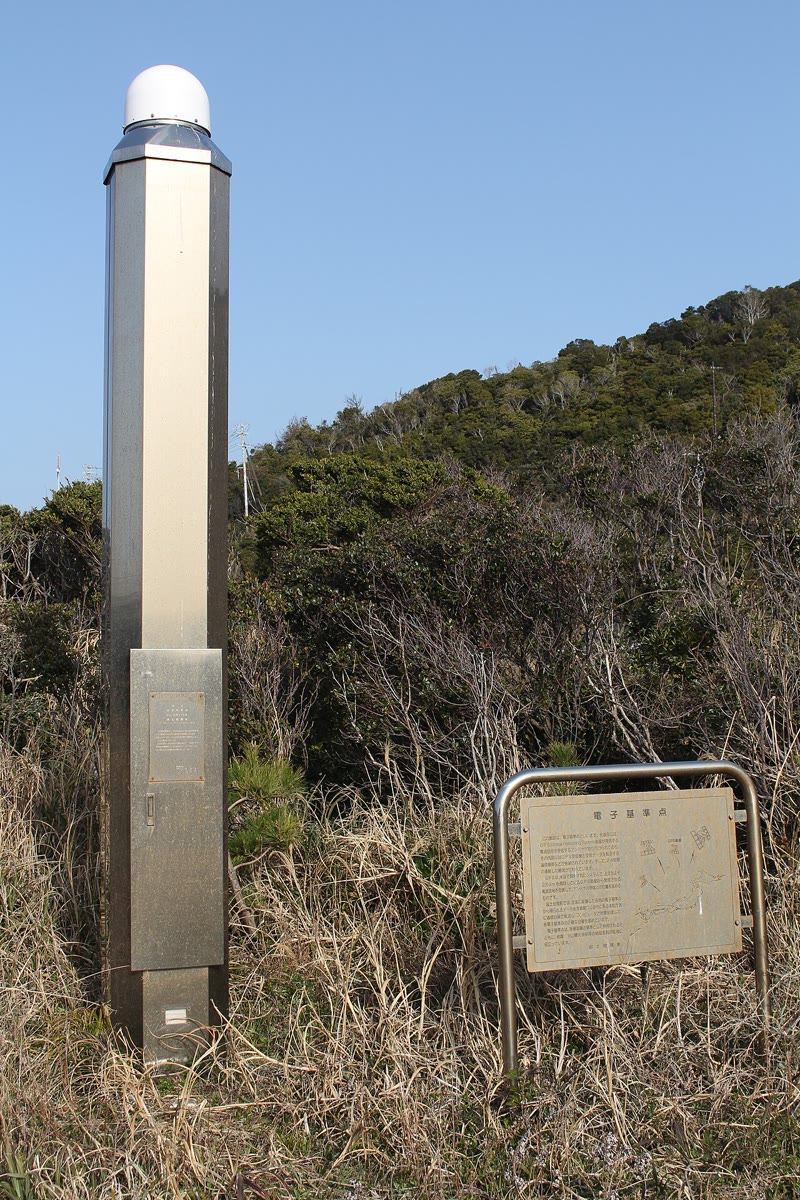
\includegraphics[width=\linewidth]{images/book3/b1-gnss-station.jpg}

{\scriptsize जापान का एक \omterm{def:b1:plate-kinematics:triple-junction}{स्थायी} स्टेशन, उसका एंटीना गुंबद के नीचे (Alpsdake, CC BY-SA 4.0)।}
\end{minipage}
\end{inthefield}

दो प्लेटों के भीतरी भागों में स्टेशनों के वेग उनका अपना \omterm{def:b1:plate-kinematics:euler-pole}{यूलर सदिश} देते हैं, भूवैज्ञानिक अभिलेख से स्वतंत्र। यूरेशिया के उत्तरी अमेरिका के सापेक्ष, ऐसा सदिश आइसलैंड में \qty{17.0}{mm.yr^{-1}} की भविष्यवाणी करता है, जो \qty{3.16}{Myr} पर औसत \qty{18.6}{mm.yr^{-1}} से लगभग \qty{8}{\percent} कम है (ऊपर का चित्र)। रेक्याविक और स्टैवेंगर के बीच की जीवा, दोनों अपनी प्लेटों के स्थिर भागों पर, \qty{17.5}{mm.yr^{-1}} से लंबी होती है; उपग्रह सदिश \qty{17.1}{mm.yr^{-1}} की भविष्यवाणी करता है, भूवैज्ञानिक वाला \qty{18.6}{mm.yr^{-1}}। उत्तरी अटलांटिक के आर-पार, कुछ दशकों पर मापी गई दर और तीन मिलियन वर्षों पर औसत दर एक दसवें के भीतर सहमत हैं: वहाँ प्लेटें आज लगभग उसी तरह चलती हैं जैसे लाखों वर्षों से चलती रही हैं।
% ledger: morvel:gps-eu-na, morvel:eu-na, ngl:reyk, ngl:stas (chord rates computed in calc/ch12.py)

सीमा-क्षेत्र के भीतर चित्र कम सरल है, क्योंकि स्टेशन प्लेटों से अधिक गति करते हैं। आइसलैंड के दसवें भाग से अधिक के नीचे हिम-टोपियाँ हैं, और उनमें से अधिकांश लगभग 1890 से द्रव्यमान खो रही हैं: भार घटने पर नीचे की \omterm{def:b1:layered-earth:layers}{भूपर्पटी} उठती है, और पतली होती बर्फ़ से दूर क्षैतिज रूप से खिसकती है। होफ़्न का स्टेशन, सबसे बड़ी हिम-टोपी के निकट दक्षिण-पूर्वी तट पर, \qty{12.9}{mm.yr^{-1}} से उठता है।
% ledger: spaans:iceland-gia, ngl:hofn

\section{अभ्यास}

पूरे में $R = \qty{6371}{km}$ लीजिए।

\begin{exercise}[$\star$]\label{exo:b1:plate-kinematics:1}
यूरेशिया का उत्तरी अमेरिका के सापेक्ष \omterm{def:b1:plate-kinematics:euler-pole}{यूलर सदिश} दर \qty{0.210}{\degree\per\Myr} रखता है। (क) इसे \unit{rad.yr^{-1}} और \unit{rad.s^{-1}} में बदलिए। (ख) एक पूरे चक्कर में कितना समय लगेगा? (ग) \unit{mm.yr^{-1}} में $\omega R$ परिकलित कीजिए।
% ledger: morvel:eu-na
\end{exercise}

\begin{exercise}[$\star$]\label{exo:b1:plate-kinematics:2}
उसी \omterm{def:b1:plate-kinematics:euler-pole}{यूलर सदिश} के साथ, \omterm{def:b1:plate-kinematics:euler-pole}{यूलर ध्रुव} से \ang{30}, \ang{60} और \ang{90} पर दोनों प्लेटों की सापेक्ष चाल परिकलित कीजिए। प्लेट सीमा के किस भाग के साथ प्रसार सबसे तेज़ होगा?
\end{exercise}

\begin{exercise}[$\star$]\label{exo:b1:plate-kinematics:3}
जरामिलो सामान्य उपकालखंड \qty{1.072}{Ma} से \qty{0.988}{Ma} तक चला। (क) \qty{50}{mm.yr^{-1}} की \omterm{def:b1:plate-kinematics:spreading-rate}{अर्ध प्रसार-दर} वाले कटक के हर पार्श्व पर वह धारी कितनी चौड़ी है? \qty{10}{mm.yr^{-1}} की? (ख) वर्तमान सामान्य कालखंड, जो \qty{0.781}{Ma} पर आरंभ हुआ, उसकी धारी की कुल चौड़ाई, \qty{10}{mm.yr^{-1}} की अर्ध दर वाले कटक पर, क्या है?
% ledger: iodp:gpts2004
\end{exercise}

\begin{exercise}[$\star$]\label{exo:b1:plate-kinematics:4}
एक कटक के आर-पार एक परिच्छेदिका पर, कालखंड C2An की विसंगति का युवा किनारा, जो \qty{2.581}{Ma} पुराना है, अक्ष के पश्चिम में \qty{66}{km} और उसके पूर्व में \qty{64}{km} है। दोनों अर्ध प्रसार-दरें और \omterm{def:b1:plate-kinematics:spreading-rate}{पूर्ण प्रसार-दर} परिकलित कीजिए। क्या प्रसार सममित है?
% ledger: iodp:gpts2004
\end{exercise}

\begin{exercise}[$\star\star$]\label{exo:b1:plate-kinematics:5}
महासागर के आर्कटिक भाग में गाक्कल कटक का एक बिंदु \ang{85}\,N, \ang{0}\,E पर है। यूरेशिया–उत्तरी अमेरिका \omterm{def:b1:plate-kinematics:euler-pole}{यूलर ध्रुव} (\ang{61.8}\,N, \ang{139.6}\,E, \qty{0.210}{\degree\per\Myr}) से उसकी कोणीय दूरी और वहाँ की प्रसार-दर परिकलित कीजिए। मापी गई \qtyrange{11}{12}{mm.yr^{-1}} दरों से तुलना कीजिए।
% ledger: morvel:eu-na
\end{exercise}

\begin{exercise}[$\star\star$]\label{exo:b1:plate-kinematics:6}
अज़ोरेस \omterm{def:b1:plate-kinematics:triple-junction}{त्रि-संधि} पर, \ang{39.44}\,N, \ang{29.83}\,W, (क) यूरेशिया–उत्तरी अमेरिका \omterm{def:b1:plate-kinematics:euler-pole}{यूलर ध्रुव} से कोणीय दूरी, (ख) प्रसार-दर, और (ग) सापेक्ष गति का दिगंश परिकलित कीजिए। (घ) संधि के ठीक उत्तर के कटक के रूपांतर भ्रंशों के लिए आप कौन-सी प्रवृत्ति की भविष्यवाणी करते हैं?
% ledger: morvel:eu-na, morvel:azores
\end{exercise}

\begin{exercise}[$\star\star$]\label{exo:b1:plate-kinematics:7}
(क) \omterm{def:b1:plate-kinematics:euler-pole}{यूलर सदिश} $\vec\omega_{\mathrm{EU\,NA}}$ (\ang{61.8}\,N, \ang{139.6}\,E, \qty{0.210}{\degree\per\Myr}) और $\vec\omega_{\mathrm{NB\,NA}}$
(\ang{79.2}\,N, \ang{40.2}\,E, \qty{0.233}{\degree\per\Myr}) को कार्तीय घटकों में, \unit{\degree\per\Myr} में लिखिए। (ख) $\vec\omega_{\mathrm{NB\,EU}}$, उसका ध्रुव और उसकी दर निकालिए। (ग) नूबिया की यूरेशिया के सापेक्ष गति जानने का यह सबसे अच्छा तरीका क्यों है?
% ledger: morvel:eu-na, morvel:nb-na
\end{exercise}

\begin{exercise}[$\star\star$]\label{exo:b1:plate-kinematics:8}
माना $\vec e_x$ \ang{0}\,N, \ang{0}\,E की ओर, $\vec e_y$ \ang{0}\,N, \ang{90}\,E की ओर और $\vec e_z$ उत्तरी ध्रुव की ओर इंगित करता है। रॉड्रिग्ज़ के सूत्र से, $\vec e_x$ का प्रतिबिंब (क) $\vec e_z$ के परितः \ang{90} के घूर्णन, और उसके बाद $\vec e_x$ के परितः \ang{90} के घूर्णन से; (ख) उन्हीं दोनों घूर्णनों को विपरीत क्रम में लेकर परिकलित कीजिए। (ग) प्लेट के अतीत की स्थितियों की पुनर्रचना के लिए इसका क्या अर्थ है?
\end{exercise}

\begin{exercise}[$\star\star$]\label{exo:b1:plate-kinematics:9}
तीन प्लेटें A, B और C एक कटक–कटक–कटक संधि पर मिलती हैं। A के सापेक्ष, प्लेट B \qty{30}{mm.yr^{-1}} पर पूर्व की ओर चलती है और प्लेट C \qty{40}{mm.yr^{-1}} पर दक्षिण की ओर। (क) वेग-त्रिभुज बनाइए। (ख) C का B के सापेक्ष चाल और दिगंश परिकलित कीजिए। (ग) यदि B और C के बीच का कटक अपनी धुरी के लंबवत प्रसार करता है, तो उनके बीच कटक की प्रवृत्ति क्या है?
\end{exercise}

\begin{exercise}[$\star\star\star$]\label{exo:b1:plate-kinematics:10}
(क) दिखाइए कि आव्यूह $R$, जो किसी भी अक्ष के परितः कोण $\alpha$ के घूर्णन का है, उसका ट्रेस $1 + 2\cos\alpha$ है। (ख) आव्यूह
\[
  R = \begin{pmatrix} 0 & 0 & 1\\ 1 & 0 & 0\\ 0 & 1 & 0\end{pmatrix}
\]
लंबकोणीय है, सारणिक $1$ के साथ। उसकी अक्ष, \omterm{def:b1:spherical-astronomy:geographic}{अक्षांश} और \omterm{def:b1:spherical-astronomy:geographic}{देशांतर} के रूप में, और उसका कोण ज्ञात कीजिए। (ग) $R$ को $\vec e_x$, $\vec e_y$
और $\vec e_z$ पर लागू करके अपने उत्तर की जाँच कीजिए।
\end{exercise}

\begin{exercise}[$\star\star\star$]\label{exo:b1:plate-kinematics:11}
उपग्रह स्थिति-निर्धारण से पहले, \omterm{def:b1:plate-kinematics:euler-pole}{यूलर ध्रुव} रूपांतर भ्रंशों की प्रवृत्तियों से खोजे जाते थे। (क) दिखाइए कि \omterm{def:b1:plate-kinematics:euler-pole}{यूलर ध्रुव} उस \omterm{def:b1:spherical-astronomy:spherical-triangle}{महावृत्त} पर स्थित है जो एक रूपांतर भ्रंश के एक बिंदु से होकर जाता है और वहाँ भ्रंश के लंबवत है, और इसलिए ध्रुव $\vec t_1\times\vec t_2$ के अनुदिश है, जहाँ $\vec t_1$ और $\vec t_2$ एक ही सीमा के दो रूपांतर भ्रंशों के अनुदिश इकाई सदिश हैं। (ख) रूपांतर भ्रंश अज़ोरेस \omterm{def:b1:plate-kinematics:triple-junction}{त्रि-संधि} के निकट \ang{95} पर (\ang{39.44}\,N, \ang{29.83}\,W) और आइसलैंड में \ang{103} पर (\ang{64.5}\,N, \ang{18}\,W) चलते हैं। \omterm{def:b1:spherical-astronomy:geographic}{अक्षांश} $\varphi$ और \omterm{def:b1:spherical-astronomy:geographic}{देशांतर} $\lambda$ पर दिगंश $\beta$ की ओर इंगित करने वाला क्षैतिज इकाई सदिश $\sin\beta\,\vec e +
\cos\beta\,\vec n$ है, जहाँ $\vec e = (-\sin\lambda, \cos\lambda, 0)$ और $\vec n =
(-\sin\varphi\cos\lambda, -\sin\varphi\sin\lambda, \cos\varphi)$। ध्रुव ज्ञात कीजिए। (ग) दो रूपांतर ध्रुव को कितनी अच्छी तरह निर्धारित करते हैं?
% ledger: morvel:eu-na
\end{exercise}

\begin{exercise}[$\star\star\star$]\label{exo:b1:plate-kinematics:12}
एक स्टेशन की पूर्वी स्थिति, हर तीन महीने पर, तीन वर्षों तक, है (मिलीमीटर में, $t = 0$ से):
\begin{center}\small
\begin{tabular}{l*{13}{c}}
\hline
$t$ (yr) & 0 & 0.25 & 0.5 & 0.75 & 1 & 1.25 & 1.5 & 1.75 & 2 & 2.25 & 2.5 & 2.75 & 3\\
$x$ (mm) & 4 & 5 & 6 & 15 & 24 & 25 & 26 & 65 & 74 & 75 & 76 & 85 & 94\\
\hline
\end{tabular}
\end{center}
यह एक स्थिर गति, एक मौसमी दोलन और एक भूकंप से हुई छलांग से बना है। (क) पहली और अंतिम स्थितियों से वेग परिकलित कीजिए। (ख) ठीक एक वर्ष के अंतर पर स्थितियों के नौ अंतर, और उनकी माध्यिका परिकलित कीजिए। (ग) एक-वर्षीय अंतरों की माध्यिका स्थिर वेग का एक मज़बूत आकलन क्यों है, और वह कब विफल होगी?
\end{exercise}

\section{समस्या: आइसलैंड का विभाजन}

\begin{problem}[{सप्ताहांत समस्या --- आइसलैंड के आर-पार उत्तरी अटलांटिक का खुलना, तीन तरीकों से मापा गया}]
\label{pb:b1:plate-kinematics:1}
% values: calc/ch12.py (Part II profile invented for the problem; real Euler
% vectors, chron ages and station velocities)
% ledger: morvel:eu-na, morvel:nb-na, iodp:gpts2004, ngl:reyk, ngl:stas, ngl:hofn
आइसलैंड मध्य-अटलांटिक कटक पर स्थित है, पश्चिम में उत्तरी अमेरिकी प्लेट और पूर्व में यूरेशियन प्लेट के बीच। $R = \qty{6371}{km}$ लीजिए और, यूरेशिया के उत्तरी अमेरिका के सापेक्ष, वह \omterm{def:b1:plate-kinematics:euler-pole}{यूलर सदिश} जिसका ध्रुव \ang{61.8}\,N, \ang{139.6}\,E पर है और दर \qty{0.210}{\degree\per\Myr} है।

\medskip
\noindent\textbf{भाग I --- प्लेट सदिश।}
\begin{enumerate}
  \item दर को \unit{rad.yr^{-1}} में बदलिए और \unit{mm.yr^{-1}} में $\omega R$ परिकलित कीजिए।
  \item ध्रुव से आइसलैंड के केंद्र, \ang{64.5}\,N, \ang{18}\,W, तक की कोणीय दूरी $\Delta$ परिकलित कीजिए।
  \item प्लेट सदिश द्वारा भविष्यवाणी की गई आइसलैंड के आर-पार \omterm{def:b1:plate-kinematics:spreading-rate}{पूर्ण प्रसार-दर} निकालिए।
  \item आइसलैंड से देखे गए ध्रुव का दिगंश, और उत्तरी अमेरिका के सापेक्ष यूरेशिया की गति का दिगंश परिकलित कीजिए।
  \item इस वेग को उसके पूर्वी और उत्तरी घटकों में विभाजित कीजिए।
  \item गाक्कल कटक पर, \ang{86}\,N, \ang{60}\,E पर, वही सदिश कौन-सी दर देता है? वहाँ सीमा इतनी धीमी क्यों है?
\end{enumerate}

\noindent\textbf{भाग II --- चुंबकीय धारियाँ।}
रेक्यनीस कटक के आर-पार, आइसलैंड के दक्षिण-पश्चिम में \ang{63}\,N, \ang{23}\,W के निकट, प्रसार की दिशा में चली एक जहाज़ की चुंबकीय परिच्छेदिका, तीन कालखंड-सीमाओं की अक्ष से दूरियाँ देती है (इस समस्या के लिए गढ़ी गई एक परिच्छेदिका):
\begin{center}\small
\begin{tabular}{lccc}
\hline
सीमा & आयु (Ma) & अक्ष के पश्चिम (km) & अक्ष के पूर्व (km)\\
\hline
C1n का आधार & 0.781 & 9.7 & 10.1\\
C2An का युवा किनारा & 2.581 & 26.8 & 27.3\\
C5n का युवा किनारा & 9.779 & 94 & 97\\
\hline
\end{tabular}
\end{center}
\begin{enumerate}[resume]
  \item C5n के युवा किनारे से, दोनों अर्ध प्रसार-दरें परिकलित कीजिए।
  \item \qty{9.8}{Ma} से \omterm{def:b1:plate-kinematics:spreading-rate}{पूर्ण प्रसार-दर} निकालिए।
  \item दोनों युवा सीमाओं से भी पूर्ण दर परिकलित कीजिए। क्या तीनों सहमत हैं? वे सीमा की आयु के साथ कैसे बदलती हैं, वर्णन कीजिए।
  \item क्या प्रसार सममित है? क्या असममिति पूर्ण दर बदलती है?
  \item रेक्यनीस कटक पर, धारियों के बीच की सीमाएँ अक्ष से दूर कुल मिलाकर, दोनों पार्श्वों को मिलाकर, \qty{5.0}{km} विस्थापित हैं। तीनों पूर्ण दरें सुधारिए। सबसे युवा सीमा के लिए सुधार सबसे अधिक क्यों मायने रखा?
  \item जरामिलो उपकालखंड (\qtyrange{1.072}{0.988}{Ma}) की धारी प्रत्येक पार्श्व पर, सुधारी अर्ध दर पर, कितनी चौड़ी है? प्रश्न 11 के विस्थापन से तुलना कीजिए। जरामिलो विसंगति रेक्यनीस कटक की परिच्छेदिकाओं पर फिर भी स्पष्ट पहचानी जाती है, पर गाक्कल कटक पर अनुपस्थित है: यह क्या सुझाता है?
  \item प्लेट सदिश परिच्छेदिका पर \qty{19.0}{mm.yr^{-1}} की भविष्यवाणी करता है। अपनी सुधारी दरों से तुलना कीजिए।
\end{enumerate}

\noindent\textbf{भाग III --- उपग्रह।}
\omterm{def:b1:plate-kinematics:triple-junction}{स्थायी} स्टेशन REYK (रेक्याविक, \ang{64.139}\,N, \ang{21.955}\,W) और STAS (स्टैवेंगर, \ang{59.018}\,N, \ang{5.599}\,E) उत्तरी अमेरिकी और यूरेशियन प्लेटों पर स्थित हैं। उनके मापे गए वेग उनके बीच की जीवा को \qty{17.5}{mm.yr^{-1}} से लंबा करते हैं।
\begin{enumerate}[resume]
  \item दोनों स्टेशनों के बीच की कोणीय दूरी, और जीवा की लंबाई परिकलित कीजिए।
  \item जीवा को एक मीटर लंबा होने में कितना समय लगता है?
  \item प्लेट सदिश STAS को उत्तरी अमेरिका के सापेक्ष \ang{114.8} की ओर \qty{18.9}{mm.yr^{-1}} का वेग देता है। REYK से \omterm{def:b1:spherical-astronomy:spherical-triangle}{महावृत्त} STAS पर \ang{123.1} की ओर पहुँचता है। इस दिशा के अनुदिश वेग का घटक परिकलित कीजिए, फिर जीवा की भविष्यवाणित लंबाई, जो STAS पर क्षैतिज के साथ कोण $\Delta/2$ बनाती है।
  \item मापी गई और भविष्यवाणित लंबाई की तुलना कीजिए। अंतर क्या समझा सकता है?
  \item उत्तरी अमेरिका के सापेक्ष REYK \qty{1.07}{mm.yr^{-1}} पश्चिम की ओर और \qty{0.97}{mm.yr^{-1}} दक्षिण की ओर चलता है, और स्टेशन HOFN (होफ़्न, दक्षिण-पूर्वी आइसलैंड) \qty{21.12}{mm.yr^{-1}} पूर्व की ओर और \qty{6.97}{mm.yr^{-1}} दक्षिण की ओर। REYK के सापेक्ष HOFN की चाल और दिगंश परिकलित कीजिए।
  \item भाग I से तुलना कीजिए। HOFN \qty{12.9}{mm.yr^{-1}} से भी उठता है। आइसलैंड के भीतर के स्टेशन प्लेट गति का खराब माप क्यों हैं?
\end{enumerate}

\noindent\textbf{भाग IV --- दस मिलियन वर्ष, और दक्षिण की संधि।}
\begin{enumerate}[resume]
  \item \qty{10}{Myr} में, यूरेशिया ध्रुव के परितः उत्तरी अमेरिका के सापेक्ष किस कोण से घूमता है?
  \item उस समय में आइसलैंड के बीच में यूरेशिया का एक बिंदु अपने लघुवृत्त पर कितनी दूरी चलता है? भाग II में C5n के युवा किनारे के बाद बनी \omterm{def:b1:layered-earth:layers}{भूपर्पटी} की सुधारी चौड़ाई से तुलना कीजिए।
  \item अज़ोरेस \omterm{def:b1:plate-kinematics:triple-junction}{त्रि-संधि} पर, प्लेट सदिश यूरेशिया को \qty{22.9}{mm.yr^{-1}} \ang{95.1} की ओर और नूबिया को \qty{19.2}{mm.yr^{-1}} \ang{103.8} की ओर देते हैं, दोनों उत्तरी अमेरिका के सापेक्ष। नूबिया के सापेक्ष यूरेशिया का वेग परिकलित कीजिए।
  \item क्या यह संधि \omterm{def:b1:plate-kinematics:triple-junction}{स्थायी} है? प्रश्न 22 का वेग यूरेशिया और नूबिया के बीच किस प्रकार की सीमा का तात्पर्य देता है?
  \item भाग I, II और III की प्रसार-दरें एकत्र कीजिए। कौन-सी सहमत हैं, और कौन-सी विधि सबसे कम समय में प्लेटों की गति मापती है?
  \item एक मिलीमीटर प्रति वर्ष तक पूर्णांकित, आइसलैंड के आर-पार कौन-सी \omterm{def:b1:plate-kinematics:spreading-rate}{पूर्ण प्रसार-दर} प्लेट सदिश और सुधारी चुंबकीय धारियाँ दोनों देती हैं?
\end{enumerate}
\end{problem}
